\section{Τεχνολογική στοίβα} \label{section:3-2-technology-stack}

Ξεκινώντας τη σχεδίαση της πλατφόρμας, πραγματοποιήθηκε έρευνα για την επιλογή της τεχνολογικής της στοίβας (technology stack). Αυτή αποφασίστηκε να ακολουθήσει μία προσαρμοσμένη για τα δεδομένα μορφή τριμερούς διάταξης\footnote{Η τριμερής διάταξη (three-tier architecture) διαχωρίζει μία εφαρμογή σε τρία ανεξάρτητα λειτουργικά επίπεδα και αποτελεί την κυρίαρχη επιλογή για διατάξεις παραδοσιακών εφαρμογών πελάτη-εξυπηρετητή.} και να χωριστεί σε τρία λογικά επίπεδα (tiers):

\begin{enumerate}
    \item \textbf{Presentation tier}: Αποτελεί τη διεπαφή του χρήστη (user interface ή UI), μέσω της οποίας ο τελευταίος αλληλεπιδρά με την εφαρμογή. Για την εκπλήρωση των προδιαγραφών, το μοναδικό απαραίτητο χαρακτηριστικό αυτού του τμήματος είναι να μπορεί να εκτελείται αυτούσιο από τη συσκευή του τελικού χρήστη, δηλαδή να μην απαιτείται η ύπαρξη κάποιου εξυπηρετητή για τη λειτουργία του. Λαμβάνοντας, επιπροσθέτως, υπόψιν τις ανάγκες και τους περιορισμούς των λογισμικών των άλλων δύο επιπέδων, το παρόν κομμάτι αποφασίστηκε να σχεδιαστεί ως μία client-side web application σε HTML/CSS/JS.

    \item \textbf{Application tier}: Πρόκειται για το επίπεδο που πραγματοποιεί την επεξεργασία (processing) της εφαρμογης. Εδώ επιλέχθηκαν το blockchain και τα smart contracts, καθώς τα θετικά τους χαρακτηριστικά, όπως αυτά περιγράφηκαν στο κεφάλαιο \ref{chapter:2-theoretical-background}, ταίριαξαν απόλυτα με τις ιδιαίτερες απαιτήσεις της εφαρμογής. Συγκεκριμένα, επιλέχθηκε η πλατφόρμα του Ethereum, καθώς αποτελεί τον πρωτοπόρο στο χώρο, με λειτουργικές εφαρμογές και την ισχυρότερη κοινότητα.

    \item \textbf{Data tier}: Το τμήμα αυτό είναι υπεύθυνο για την αποθήκευση των δεδομένων (storage). Για την επίτευξη πλήρους αρχιτεκτονικής αποκέντρωσης των δεδομένων επιλέχθηκε το IPFS (ενότητα \ref{section:2-7-ipfs}), το οποίο διανέμει το περιεχόμενο της εφαρμογής στους peers που συμμετέχουν σε αυτήν.
\end{enumerate}

Τελικά, με τη διασύνδεση των προαναφερθέντων τεχνολογιών, προκύπτει σχηματικά η ακόλουθη διάταξη:

% TODO: change this
\begin{figure}[H]
    \centering
    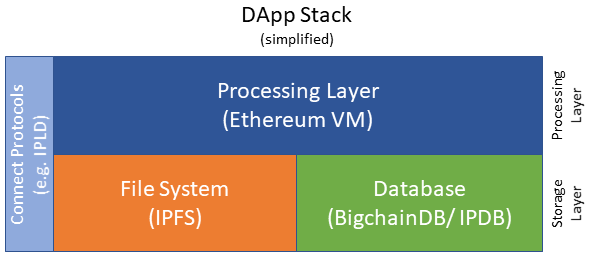
\includegraphics[width=.75\textwidth]{assets/figures/chapter-3/simple_dapp_stack}
    \caption{Τεχνολογική στοίβα}
\end{figure}
